%----------------------------------------------------------------------------------------
%	PACKAGES AND THEMES
%----------------------------------------------------------------------------------------

\documentclass{beamer}

\mode<presentation> {
\usetheme{Madrid}
}

\usepackage{graphicx}
\usepackage{booktabs}
\usepackage{polski}
\usepackage[polish]{babel}
\usepackage[utf8]{inputenc}
\usepackage[T1]{fontenc}
\usepackage[utf8]{luainputenc}
\usepackage{pgfgantt}
\usepackage{caption}
\usepackage{mwe}

% Strona tytułowa
\usepackage{pgfplots}
\usepackage{siunitx}
\usepackage{paracol}
\usepackage{gensymb}

% Pływające obrazki
\usepackage{float}
\usepackage{svg}
\usepackage{graphicx}
\usepackage{subfig}


\sisetup{group-digits=true,
        %  group-four-digits=true,
        round-precision=4,
        group-separator={},
        output-decimal-marker={,}}

\DeclareCaptionFormat{citation}{%
   \ifx\captioncitation\relax\relax\else
     \captioncitation\par
   \fi
   #1#2#3\par}
\newcommand*\setcaptioncitation[1]{\def\captioncitation{\tiny{\textit{Źródło:}~#1}\medskip}\normalsize}
\let\captioncitation\relax
\captionsetup{format=citation,justification=centering}

\usetikzlibrary{pgfplots.groupplots}
\sisetup{detect-weight,exponent-product=\cdot,output-decimal-marker={,},per-mode=symbol,binary-units=true,range-phrase={-},range-units=single}

%wymiar tekstu
\def\figurename{Rys.}
\def\tablename{Tab.}

%----------------------------------------------------------------------------------------
%	TITLE PAGE
%----------------------------------------------------------------------------------------

\title[Metody Identyfikacji - Projekt]{Metody Identyfikacji}

\author{Radosław Gryta \and Jakub Sikora} 
\date{1 czerwca 2020}
\institute[]{
  Modelowanie poziomu wody w walczaku \\
  oraz podciśnienia w komorze spalania \\ 
  w instalacji przemysłowego kotła grzewczego
}
\AtBeginSection[]
{
    \begin{frame}[plain, noframenumbering]
        \frametitle{Agenda}
        \tableofcontents[currentsection]
    \end{frame}
}

\begin{document}

\begin{frame}
\titlepage
\end{frame}

%----------------------------------------------------------------------------------------
%	PRESENTATION SLIDES
%----------------------------------------------------------------------------------------

\begin{frame}[plain,c]
  \begin{center}
    \Huge Model ARX
  \end{center}
\end{frame}

\begin{frame}
  \frametitle{Model ARX- zasada działania}
  \begin{block}{Założenia:}
    \begin{itemize}
      \item dobranie wejść modelu przy pomocy współczynnika korelacji,
        \begin{itemize}
          \item weryfikacja skrośna wszystkich zestawów danych,
          \item dobranie na podstawie jednego zestawu, 
        \end{itemize}
      \item dobranie stopni wielomianów modelu przy pomocy algorytmu genetycznego (ga),
      \item wyznaczenie parametrów modelu ARX wykorzystując MNK przy wcześniejszym ustaleniu liczby wejść.
    \end{itemize}
  \end{block}

  \begin{block}{Dla przychodzącego zestawu wejść:}
    \begin{itemize}
      \item wykorzystanie danych historycznych,
      \item przemnożenie przez wektor wyznaczonych parametrów. 
    \end{itemize}
  \end{block}
\end{frame}

\begin{frame}
  \frametitle{Model ARX - przygotowanie danych i uczenie modelu}
  \begin{block}{Operacja wykonywane na danych uczących}
    \begin{itemize}
      \item wyznaczenie sygnałów wejściowych na podstawie współczynnika korelacji,
      \item interpolacja/usunięcie próbek brakujących/nadmiarowych,
      \item podział danych na zestawy,
      \begin{itemize}
        \item uczący (z. 1 oraz z. 2),
        \item weryfikujący (z. 3 oraz z. 4).
      \end{itemize}
    \end{itemize}
  \end{block}

  \begin{block}{Proces uczenia modelu:}
    \begin{itemize}
      \item dobranie współczynnika minimalnej korelacji,
      \item na podstawie wyznaczonych wejść opracowanie modelu wstępnego arx z danych uczących,
      \item sprawdzenie poprawności modelu na podstawie zestawu weryfikującego.
    \end{itemize}
  \end{block}
\end{frame}



\begin{frame}
  \frametitle{Działanie modelu ARX dla sygnału LT01}
  \begin{figure}[H]
    \centering
    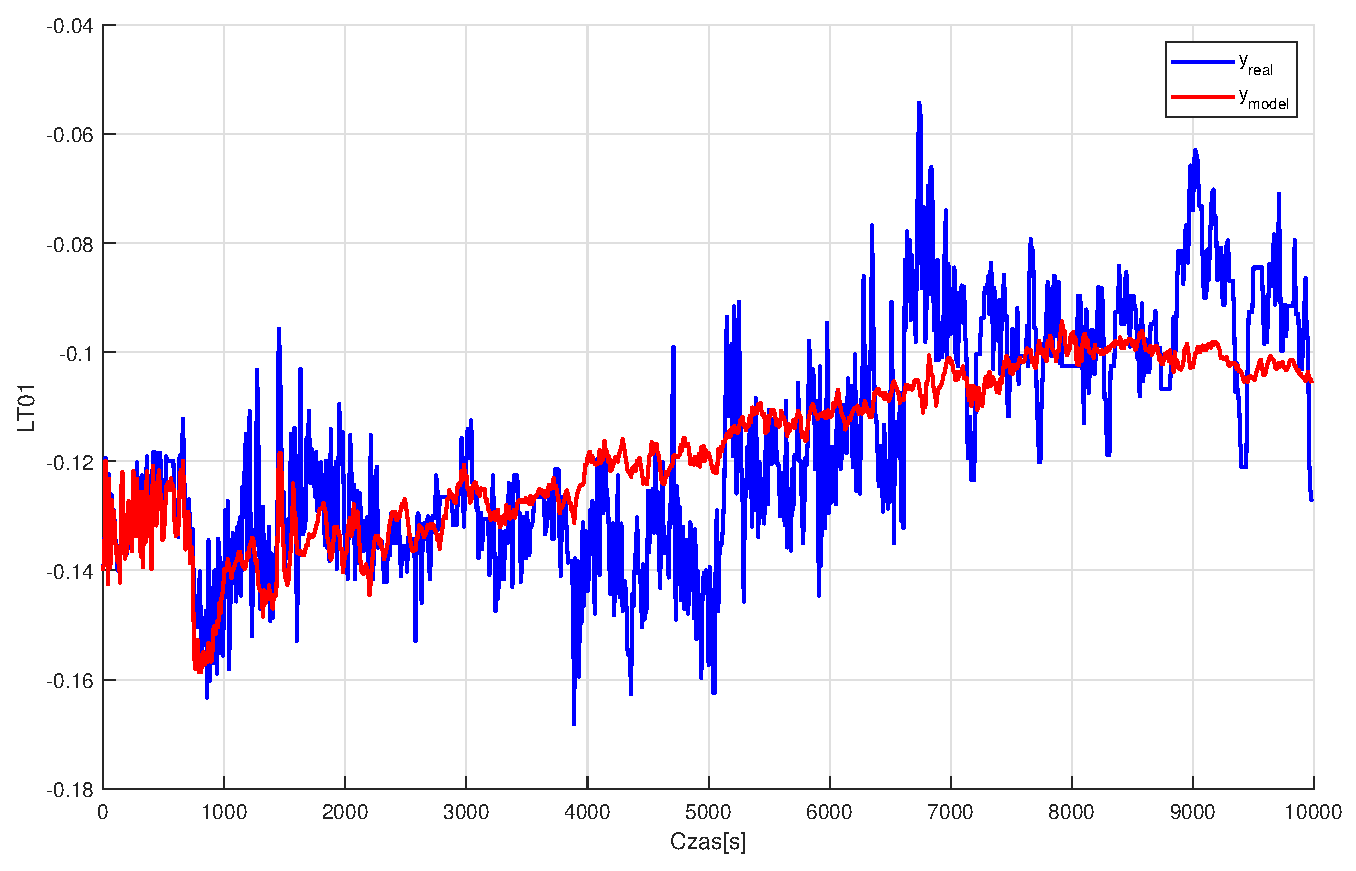
\includegraphics[width=0.75\linewidth,keepaspectratio]{results_matlab/LT01_1.eps}
    \caption{Porównanie działania modelu ARX z danymi uczącymi (z. 1)}
    \label{fig:test}
    \end{figure}
\end{frame}

\addtocounter{framenumber}{-1}
\begin{frame}
  \frametitle{Działanie modelu ARX dla sygnału LT01}
  \begin{figure}[H]
    \centering
    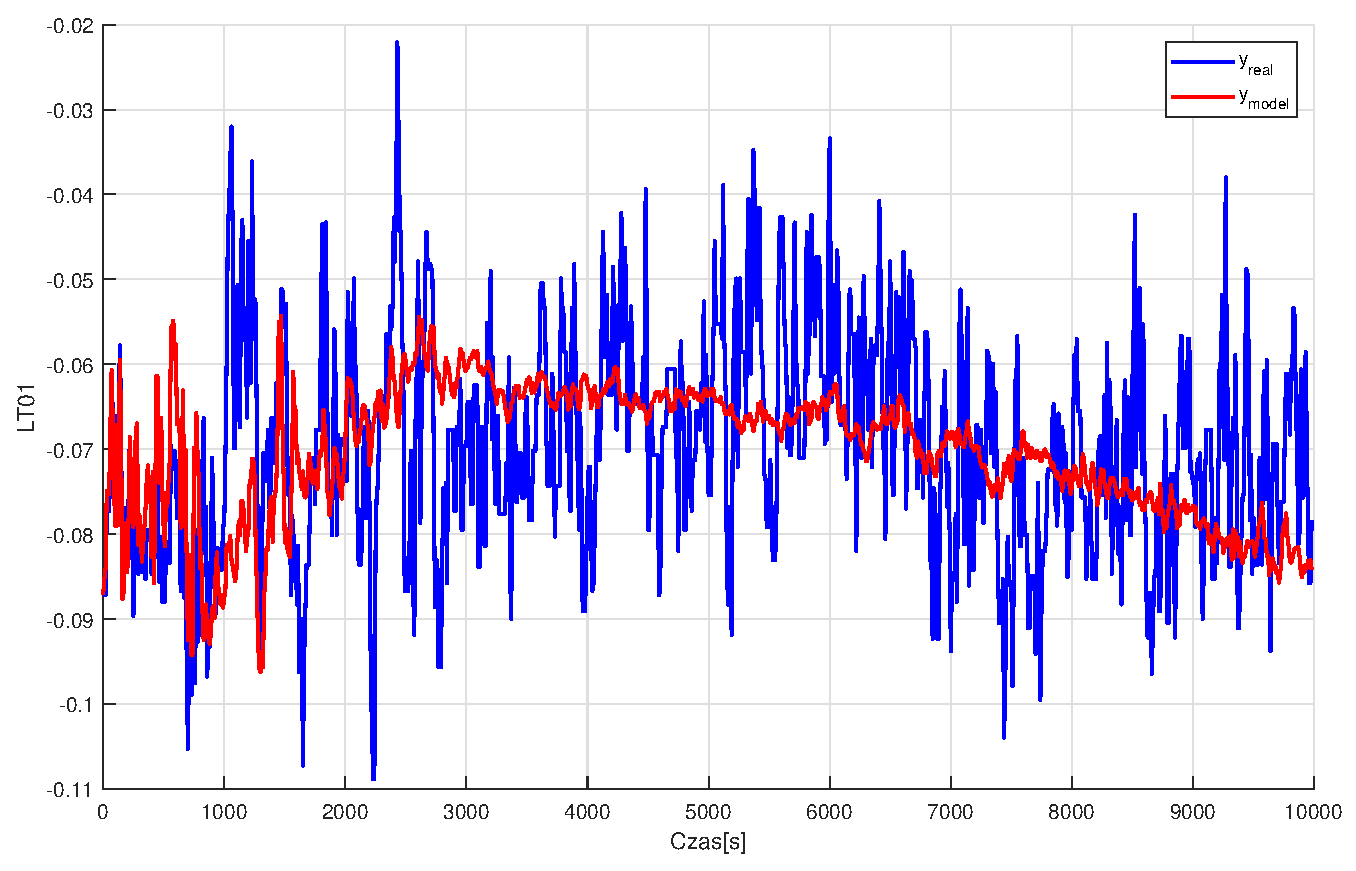
\includegraphics[width=0.75\linewidth,keepaspectratio]{results_matlab/LT01_2.eps}
    \caption{Porównanie działania modelu ARX z danymi uczącymi (z. 2)}
    \label{fig:test}
    \end{figure}
\end{frame}

\addtocounter{framenumber}{-1}
\begin{frame}
  \frametitle{Działanie modelu ARX dla sygnału LT01}
  \begin{figure}[H]
    \centering
    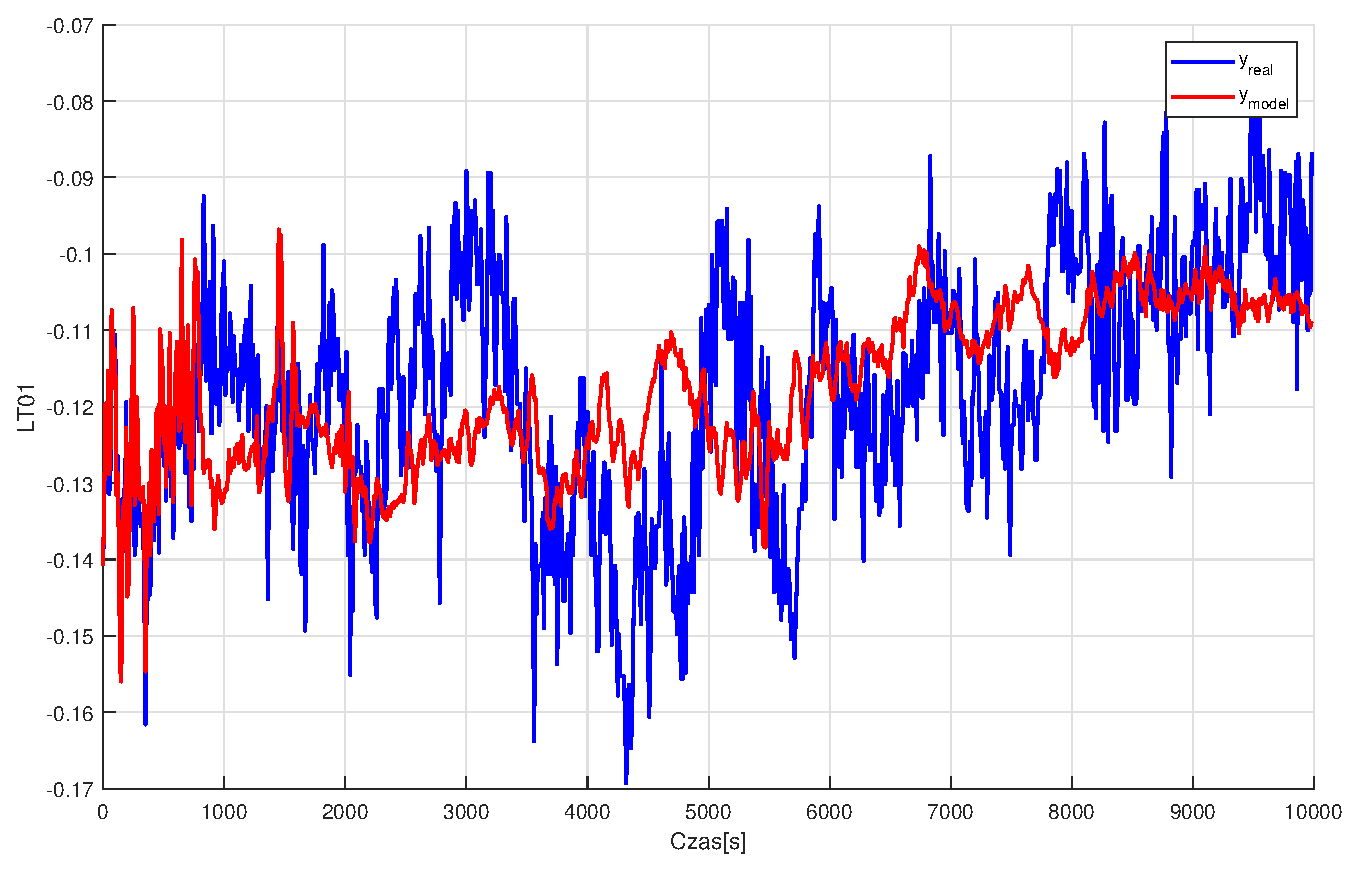
\includegraphics[width=0.75\linewidth,keepaspectratio]{results_matlab/LT01_3.eps}
    \caption{Porównanie działania modelu ARX z danymi weryfikacyjnymi (z. 3)}
    \label{fig:test}
    \end{figure}
\end{frame}

\addtocounter{framenumber}{-1}
\begin{frame}
  \frametitle{Działanie modelu ARX dla sygnału LT01}
  \begin{figure}[H]
    \centering
    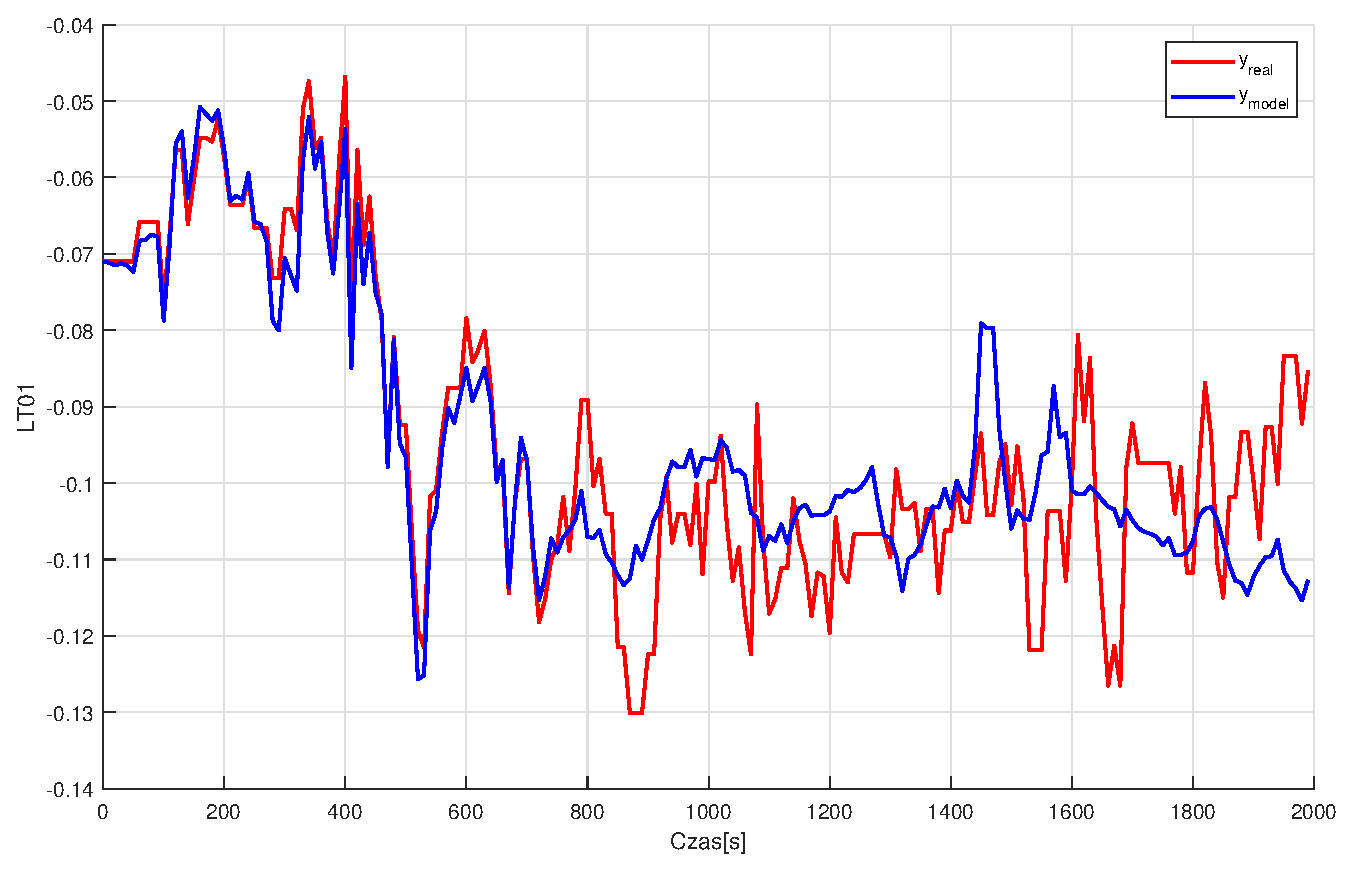
\includegraphics[width=0.75\linewidth,keepaspectratio]{results_matlab/LT01_4.eps}
    \caption{Porównanie działania modelu ARX z danymi weryfikacyjnymi (z. 4)}
    \label{fig:test}
    \end{figure}
\end{frame}

\begin{frame}
  \frametitle{Działanie modelu ARX dla sygnału DP}
  \begin{figure}[H]
    \centering
    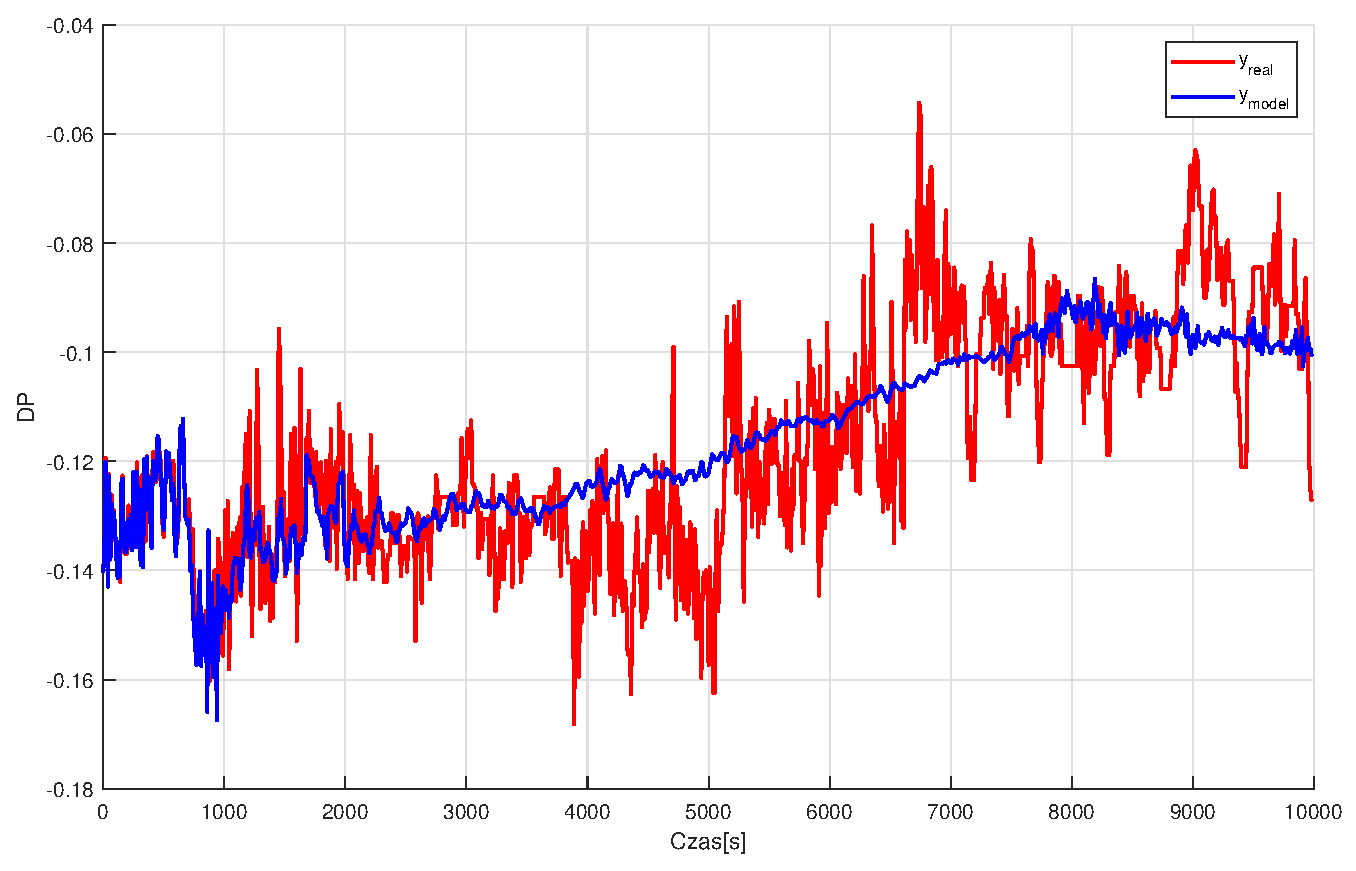
\includegraphics[width=0.75\linewidth,keepaspectratio]{results_matlab/DP_1.eps}
    \caption{Porównanie działania modelu ARX z danymi uczącymi (z. 1)}
    \label{fig:test}
    \end{figure}
\end{frame}

\addtocounter{framenumber}{-1}
\begin{frame}
  \frametitle{Działanie modelu ARX dla sygnału DP}
  \begin{figure}[H]
    \centering
    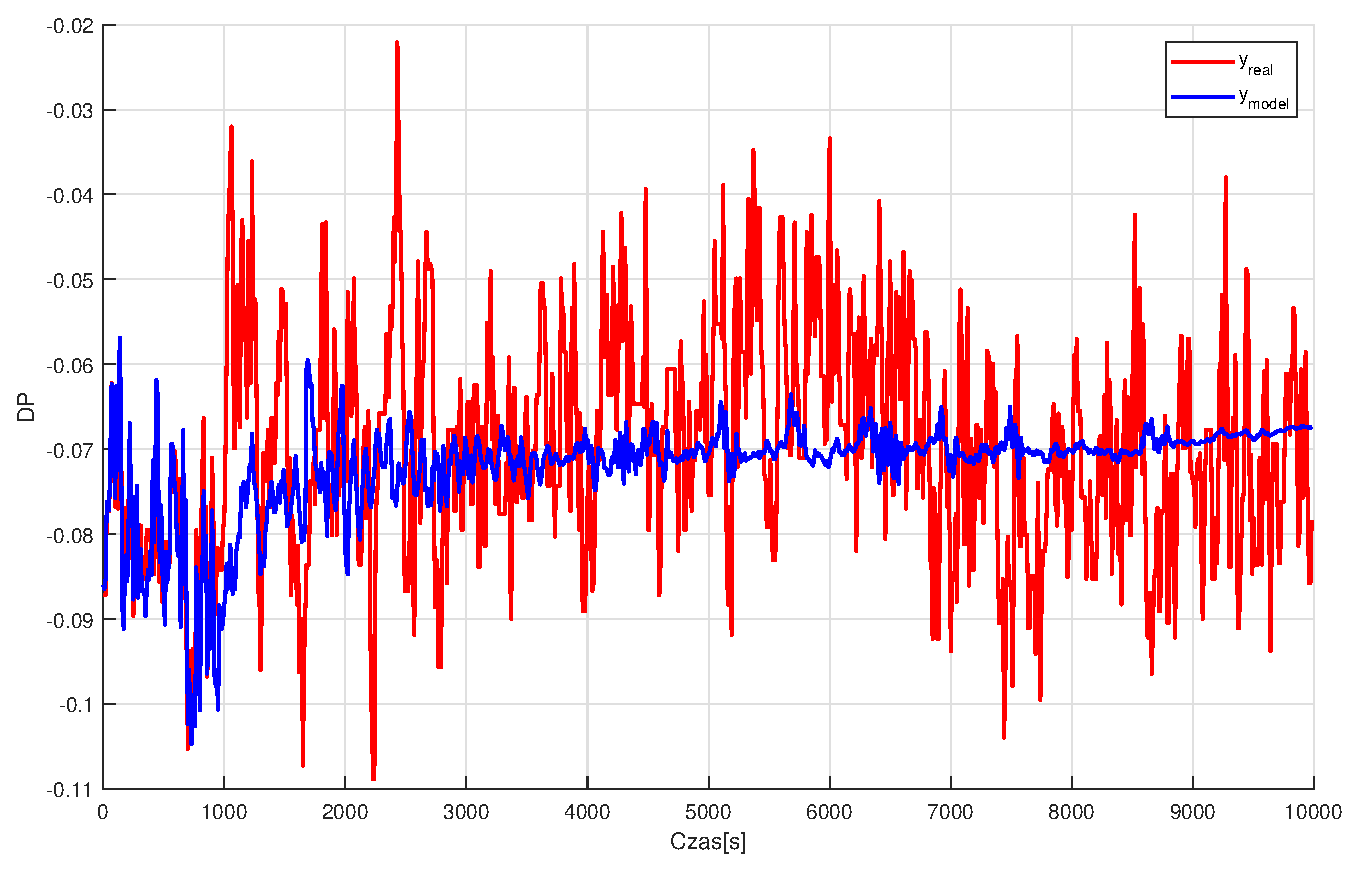
\includegraphics[width=0.75\linewidth,keepaspectratio]{results_matlab/DP_2.eps}
    \caption{Porównanie działania modelu ARX z danymi uczącymi (z. 2)}
    \label{fig:test}
    \end{figure}
\end{frame}

\addtocounter{framenumber}{-1}
\begin{frame}
  \frametitle{Działanie modelu ARX dla sygnału DP}
  \begin{figure}[H]
    \centering
    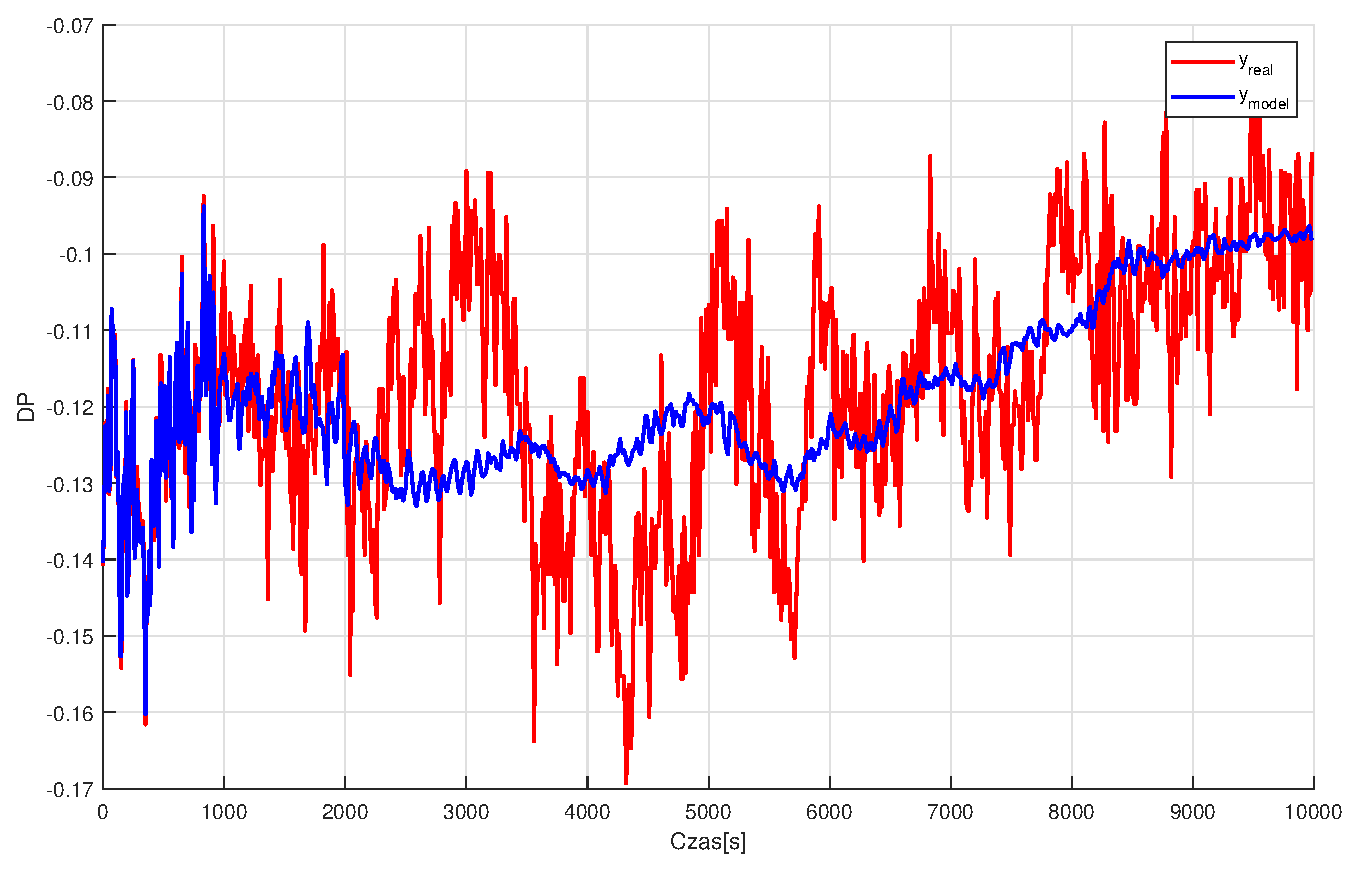
\includegraphics[width=0.75\linewidth,keepaspectratio]{results_matlab/DP_3.eps}
    \caption{Porównanie działania modelu ARX z danymi weryfikacyjnymi (z. 3)}
    \label{fig:test}
    \end{figure}
\end{frame}

\addtocounter{framenumber}{-1}
\begin{frame}
  \frametitle{Działanie modelu ARX dla sygnału DP}
  \begin{figure}[H]
    \centering
    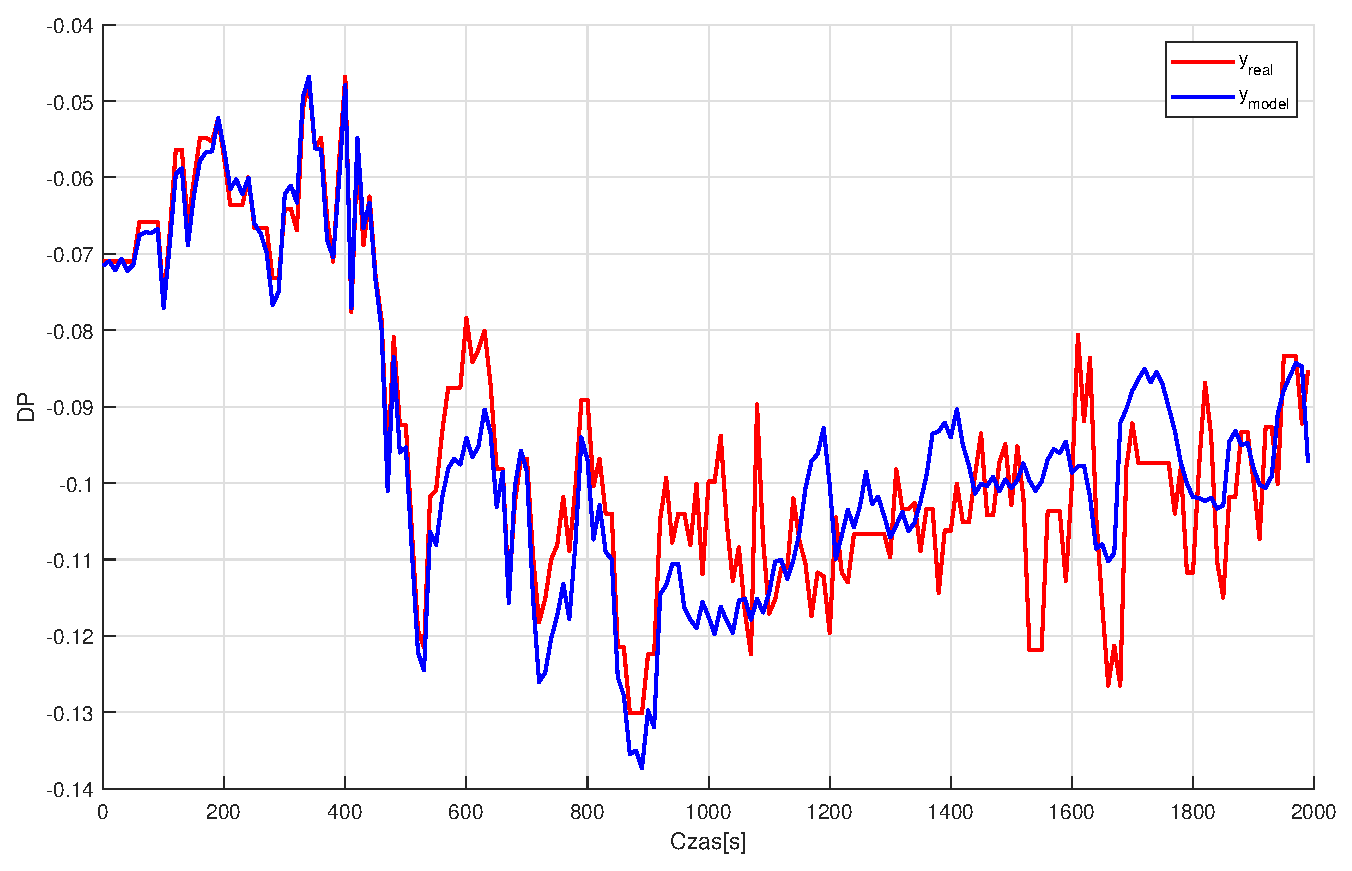
\includegraphics[width=0.75\linewidth,keepaspectratio]{results_matlab/DP_4.eps}
    \caption{Porównanie działania modelu ARX z danymi weryfikacyjnymi (z. 4)}
    \label{fig:test}
    \end{figure}
\end{frame}

\begin{frame}
  \frametitle{Model ARX - wady i zalety}
  \begin{exampleblock}{Zalety}
    \begin{itemize}
      \item łatwy do nauczenia,
      \item łatwo rozszerzalny.
    \end{itemize}
  \end{exampleblock}
  \begin{alertblock}{Wady}
    \begin{itemize}
      \item wysoki koszt obliczeniowy dopasowywania parametrów modelu ARX i minimalnej wartości współczynnika korelacji,
      \item do szukania parametrów wykorzystana MNK,
      \item złożoność rośnie nieliniowo względem wejść.
    \end{itemize}
  \end{alertblock}
\end{frame}

\begin{frame}[plain,c]
  \begin{center}
    \Huge Model ES-ARMA
  \end{center}
\end{frame}


\begin{frame}
  \frametitle{Model ES-ARMA - zasada działania}
  \begin{block}{Założenia:}
    \begin{itemize}
      \item bierzemy wszystkie nieskorelowane ze sobą wejścia,
      \item opisujemy strukturę modelu za pomocą macierzy M opisującej rząd dynamiki oraz, opóźnienie danego wejścia,
      \item dobieramy wartości macierzy M (hiperparametry) za pomocą algorytmu ewolucyjnego,
      \item wartości parametrów modelu ARMA dobieramy za pomocą metody najmniejszych kwadratów.
    \end{itemize}
  \end{block}

  \begin{block}{Dla przychodzącego zestawu wejść:}
    \begin{itemize}
      \item tworzymy wektor próbek korzystając z poprzednich wejść i wyjść modelu,
      \item wymnażamy wektor próbek przez wektor parametrów. 
    \end{itemize}
  \end{block}
\end{frame}

\begin{frame}
  \frametitle{Model ES-ARMA - przygotowanie danych i uczenie modelu}
  \begin{block}{Operacja wykonywane na danych uczących}
    \begin{itemize}
      \item ujednolicenie okresu próbkowania,
      \item interpolacja brakujących danych,
      \item usunięcie skorelowanych ze sobą wejść.
    \end{itemize}
  \end{block}

  \begin{block}{Proces uczenia modelu:}
    \begin{itemize}
      \item znalezienie hiperparametrów modelu przy użyciu walidacji skrośnej,
      \begin{itemize}
        \item dla każdego zestawu danych uczymy model metodą najmniejszych kwadratów i liczymy współczynnik determinancji,
        \item średnia współczynników determinancji jest funkcją celu algorytmu ewolucyjnego,
      \end{itemize}
      \item dla każdego zestawu danych tworzymy macierz regresji, zgodną z obliczonym M,
      \item losowo wybieramy 33\% próbek z każdej z macierzy do zbioru uczącego,
      \item ostatecznie uczymy model za pomocą MNK.
    \end{itemize}
  \end{block}
\end{frame}

\begin{frame}
  \frametitle{Działanie modelu ES-ARMA dla sygnału LT01}
    \begin{figure}[t]
      \centering
      \begin{tikzpicture}
        \begin{axis}[
          ticklabel style={
          /pgf/number format/fixed,
          /pgf/number format/precision=5
          }, scaled ticks=false,
          width=0.95\textwidth,
          height=0.75\textheight,
          grid=major,
          xmin=0, xmax=9650, %ymin=-0.2, ymax=0.3,
          xlabel={$t [s]$},
          xtick={0, 2000, 4000, 6000, 8000},
          ylabel={$y(t)$},
          legend pos=north east,
          legend style={nodes={scale=0.6, transform shape}, font={\large}},
          legend image post style={mark=-}],
          y tick label style={/pgf/number format/1000 sep=},
        ]
          \addplot[red, semithick] file{ ./results/parsed/genetic/lt01_0_yverif.csv };
          \addplot[blue, semithick] file{ ./results/parsed/genetic/lt01_0_ymodel.csv };
          \addlegendentry{$y_{\mathrm{LT01}}^{\mathrm{verif}}$},
          \addlegendentry{$y_{\mathrm{LT01}}^{\mathrm{model}}$},
          \addlegendimage{no markers, red}
          \addlegendimage{no markers, blue}
        \end{axis}
      \end{tikzpicture}
      \caption{Porównanie działania modelu ES-ARMA z danymi weryfikacyjnymi (0)}
    \end{figure}
\end{frame}

\addtocounter{framenumber}{-1}
\begin{frame}
  \frametitle{Działanie modelu ES-ARMA dla sygnału LT01}
    \begin{figure}[t]
      \centering
      \begin{tikzpicture}
        \begin{axis}[
          ticklabel style={
          /pgf/number format/fixed,
          /pgf/number format/precision=5
          }, scaled ticks=false,
          width=0.95\textwidth,
          height=0.75\textheight,
          grid=major,
          xmin=0, xmax=9650, %ymin=-0.2, ymax=0.3,
          xlabel={$t [s]$},
          xtick={0, 2000, 4000, 6000, 8000},
          ylabel={$y(t)$},
          legend pos=north east,
          legend style={nodes={scale=0.6, transform shape}, font={\large}},
          legend image post style={mark=-}],
          y tick label style={/pgf/number format/1000 sep=},
        ]
          \addplot[red, semithick] file{ ./results/parsed/genetic/lt01_1_yverif.csv };
          \addplot[blue, semithick] file{ ./results/parsed/genetic/lt01_1_ymodel.csv };
          \addlegendentry{$y_{\mathrm{LT01}}^{\mathrm{verif}}$},
          \addlegendentry{$y_{\mathrm{LT01}}^{\mathrm{model}}$},
          \addlegendimage{no markers, red}
          \addlegendimage{no markers, blue}
        \end{axis}
      \end{tikzpicture}
      \caption{Porównanie działania modelu ES-ARMA z danymi weryfikacyjnymi (1)}
    \end{figure}
\end{frame}

\addtocounter{framenumber}{-1}
\begin{frame}
  \frametitle{Działanie modelu ES-ARMA dla sygnału LT01}
    \begin{figure}[t]
      \centering
      \begin{tikzpicture}
        \begin{axis}[
          ticklabel style={
          /pgf/number format/fixed,
          /pgf/number format/precision=5
          }, scaled ticks=false,
          width=0.95\textwidth,
          height=0.75\textheight,
          grid=major,
          xmin=0, xmax=9650, %ymin=-0.2, ymax=0.3,
          xlabel={$t [s]$},
          xtick={0, 2000, 4000, 6000, 8000},
          ylabel={$y(t)$},
          legend pos=north east,
          legend style={nodes={scale=0.6, transform shape}, font={\large}},
          legend image post style={mark=-}],
          y tick label style={/pgf/number format/1000 sep=},
        ]
          \addplot[red, semithick] file{ ./results/parsed/genetic/lt01_2_yverif.csv };
          \addplot[blue, semithick] file{ ./results/parsed/genetic/lt01_2_ymodel.csv };
          \addlegendentry{$y_{\mathrm{LT01}}^{\mathrm{verif}}$},
          \addlegendentry{$y_{\mathrm{LT01}}^{\mathrm{model}}$},
          \addlegendimage{no markers, red}
          \addlegendimage{no markers, blue}
        \end{axis}
      \end{tikzpicture}
      \caption{Porównanie działania modelu ES-ARMA z danymi weryfikacyjnymi (2)}
    \end{figure}
\end{frame}

\addtocounter{framenumber}{-1}
\begin{frame}
  \frametitle{Działanie modelu ES-ARMA dla sygnału LT01}
    \begin{figure}[t]
      \centering
      \begin{tikzpicture}
        \begin{axis}[
          ticklabel style={
          /pgf/number format/fixed,
          /pgf/number format/precision=5
          }, scaled ticks=false,
          width=0.95\textwidth,
          height=0.75\textheight,
          grid=major,
          xmin=0, xmax=1660, %ymin=-0.2, ymax=0.3,
          xlabel={$t [s]$},
          xtick={0, 400, 800, 1200, 1600},
          ylabel={$y(t)$},
          legend pos=south east,
          legend style={nodes={scale=0.6, transform shape}, font={\large}},
          legend image post style={mark=-}],
          y tick label style={/pgf/number format/1000 sep=},
        ]
          \addplot[red, semithick] file{ ./results/parsed/genetic/lt01_3_yverif.csv };
          \addplot[blue, semithick] file{ ./results/parsed/genetic/lt01_3_ymodel.csv };
          \addlegendentry{$y_{\mathrm{LT01}}^{\mathrm{verif}}$},
          \addlegendentry{$y_{\mathrm{LT01}}^{\mathrm{model}}$},
          \addlegendimage{no markers, red}
          \addlegendimage{no markers, blue}
        \end{axis}
      \end{tikzpicture}
      \caption{Porównanie działania modelu ES-ARMA z danymi weryfikacyjnymi (3)}
    \end{figure}
\end{frame}

\begin{frame}
  \frametitle{Działanie modelu ES-ARMA dla sygnału DP}
    \begin{figure}[t]
      \centering
      \begin{tikzpicture}
        \begin{axis}[
          ticklabel style={
          /pgf/number format/fixed,
          /pgf/number format/precision=5
          }, scaled ticks=false,
          width=0.95\textwidth,
          height=0.75\textheight,
          grid=major,
          xmin=0, xmax=9640, %ymin=-0.2, ymax=0.3,
          xlabel={$t [s]$},
          xtick={0, 2000, 4000, 6000, 8000},
          ylabel={$y(t)$},
          legend pos=south east,
          legend style={nodes={scale=0.6, transform shape}, font={\large}},
          legend image post style={mark=-}],
          y tick label style={/pgf/number format/1000 sep=},
        ]
          \addplot[red, semithick] file{ ./results/parsed/genetic/dp0_yverif.csv };
          \addplot[blue, semithick] file{ ./results/parsed/genetic/dp0_ymodel.csv };
          \addlegendentry{$y_{\mathrm{DP}}^{\mathrm{verif}}$},
          \addlegendentry{$y_{\mathrm{DP}}^{\mathrm{model}}$},
          \addlegendimage{no markers, red}
          \addlegendimage{no markers, blue}
        \end{axis}
      \end{tikzpicture}
      \caption{Porównanie działania modelu ES-ARMA z danymi weryfikacyjnymi (0)}
    \end{figure}
\end{frame}

\addtocounter{framenumber}{-1}
\begin{frame}
  \frametitle{Działanie modelu ES-ARMA dla sygnału DP}
    \begin{figure}[t]
      \centering
      \begin{tikzpicture}
        \begin{axis}[
          ticklabel style={
          /pgf/number format/fixed,
          /pgf/number format/precision=5
          }, scaled ticks=false,
          width=0.95\textwidth,
          height=0.75\textheight,
          grid=major,
          xmin=0, xmax=9650, %ymin=-0.2, ymax=0.3,
          xlabel={$t [s]$},
          xtick={0, 2000, 4000, 6000, 8000},
          ylabel={$y(t)$},
          legend pos=north east,
          legend style={nodes={scale=0.6, transform shape}, font={\large}},
          legend image post style={mark=-}],
          y tick label style={/pgf/number format/1000 sep=},
        ]
          \addplot[red, semithick] file{ ./results/parsed/genetic/dp1_yverif.csv };
          \addplot[blue, semithick] file{ ./results/parsed/genetic/dp1_ymodel.csv };
          \addlegendentry{$y_{\mathrm{DP}}^{\mathrm{verif}}$},
          \addlegendentry{$y_{\mathrm{DP}}^{\mathrm{model}}$},
          \addlegendimage{no markers, red}
          \addlegendimage{no markers, blue}
        \end{axis}
      \end{tikzpicture}
      \caption{Porównanie działania modelu ES-ARMA z danymi weryfikacyjnymi (1)}
    \end{figure}
\end{frame}

\addtocounter{framenumber}{-1}
\begin{frame}
  \frametitle{Działanie modelu ES-ARMA dla sygnału DP}
    \begin{figure}[t]
      \centering
      \begin{tikzpicture}
        \begin{axis}[
          ticklabel style={
          /pgf/number format/fixed,
          /pgf/number format/precision=5
          }, scaled ticks=false,
          width=0.95\textwidth,
          height=0.75\textheight,
          grid=major,
          xmin=0, xmax=9650, %ymin=-0.2, ymax=0.3,
          xlabel={$t [s]$},
          xtick={0, 2000, 4000, 6000, 8000},
          ylabel={$y(t)$},
          legend pos=south east,
          legend style={nodes={scale=0.6, transform shape}, font={\large}},
          legend image post style={mark=-}],
          y tick label style={/pgf/number format/1000 sep=},
        ]
          \addplot[red, semithick] file{ ./results/parsed/genetic/dp2_yverif.csv };
          \addplot[blue, semithick] file{ ./results/parsed/genetic/dp2_ymodel.csv };
          \addlegendentry{$y_{\mathrm{DP}}^{\mathrm{verif}}$},
          \addlegendentry{$y_{\mathrm{DP}}^{\mathrm{model}}$},
          \addlegendimage{no markers, red}
          \addlegendimage{no markers, blue}
        \end{axis}
      \end{tikzpicture}
      \caption{Porównanie działania modelu ES-ARMA z danymi weryfikacyjnymi (2)}
    \end{figure}
\end{frame}

\addtocounter{framenumber}{-1}
\begin{frame}
  \frametitle{Działanie modelu ES-ARMA dla sygnału DP}
    \begin{figure}[t]
      \centering
      \begin{tikzpicture}
        \begin{axis}[
          ticklabel style={
          /pgf/number format/fixed,
          /pgf/number format/precision=5
          }, scaled ticks=false,
          width=0.95\textwidth,
          height=0.75\textheight,
          grid=major,
          xmin=0, xmax=1650, %ymin=-0.2, ymax=0.3,
          xlabel={$t [s]$},
          xtick={0, 400, 800, 1200, 1600},
          ylabel={$y(t)$},
          legend pos=north east,
          legend style={nodes={scale=0.6, transform shape}, font={\large}},
          legend image post style={mark=-}],
          y tick label style={/pgf/number format/1000 sep=},
        ]
          \addplot[red, semithick] file{ ./results/parsed/genetic/dp3_yverif.csv };
          \addplot[blue, semithick] file{ ./results/parsed/genetic/dp3_ymodel.csv };
          \addlegendentry{$y_{\mathrm{DP}}^{\mathrm{verif}}$},
          \addlegendentry{$y_{\mathrm{DP}}^{\mathrm{model}}$},
          \addlegendimage{no markers, red}
          \addlegendimage{no markers, blue}
        \end{axis}
      \end{tikzpicture}
      \caption{Porównanie działania modelu ES-ARMA z danymi weryfikacyjnymi (3)}
    \end{figure}
\end{frame}

\begin{frame}
  \frametitle{Model ES-ARMA - wady i zalety}
  \begin{exampleblock}{Zalety}
    \begin{itemize}
      \item dobra dokładność,
      \item łatwe wyznaczanie kolejnego wyjścia,
      \item możliwa wymiana modelu wewnętrznego,
      \item znana struktura modelu - model parametryczny.
    \end{itemize}
  \end{exampleblock}
  \begin{alertblock}{Wady}
    \begin{itemize}
      \item kosztowny proces szukania hiperparametrów,
      \item do szukania parametrów wykorzystana MNK,
      \item złożoność rośnie nieliniowo względem wejść.
    \end{itemize}
  \end{alertblock}
\end{frame}

\begin{frame}[plain,c]
  \begin{center}
    \Huge Model KNNR
  \end{center}
\end{frame}

\begin{frame}
  \frametitle{Model KNNR - zasada działania}
  \begin{block}{Założenia:}
    \begin{itemize}
      \item modelujemy zjawisko jako proces statyczny,
      \item modelowana sytuacja musiała się już kiedyś wydarzyć,
      \item uśrednianie wielu próbek pozwoli zamodelować dynamikę,
      \item wiedza modelu jest przechowywana w~postaci par (wejścia, wyjście).
    \end{itemize}
  \end{block}

  \begin{block}{Dla przychodzącego zestawu wejść:}
    \begin{itemize}
      \item liczymy odległość Euklidesową od każdej próbki ze zbioru uczącego,
      \item wyznaczamy k najbliższych próbek,
      \item wyjściem modelu jest średnia ważona odpowiadających próbkom wyjść. 
    \end{itemize}
  \end{block}
\end{frame}

\begin{frame}
  \frametitle{Model KNNR - przygotowanie danych i uczenie modelu}
  \begin{block}{Operacja wykonywane na danych uczących}
    \begin{itemize}
      \item ujednolicenie okresu próbkowania,
      \item interpolacja brakujących danych,
      \item analiza PCA.
    \end{itemize}
  \end{block}
  \begin{block}{Proces uczenia modelu:}
    \begin{itemize}
      \item wydzielenie z każdego zestawu danych 33\% próbek uczących,
      \item agregacja danych w pamięci modelu.
    \end{itemize}
  \end{block}
\end{frame}

\begin{frame}
  \frametitle{Działanie modelu KNNR dla sygnału LT01}
    \begin{figure}[t]
      \centering
      \begin{tikzpicture}
        \begin{axis}[
          ticklabel style={
          /pgf/number format/fixed,
          /pgf/number format/precision=5
          }, scaled ticks=false,
          width=0.95\textwidth,
          height=0.75\textheight,
          grid=major,
          xmin=0, xmax=10000, %ymin=-0.2, ymax=0.3,
          xlabel={$t [s]$},
          xtick={0, 2000, 4000, 6000, 8000, 10000},
          ylabel={$y(t)$},
          legend pos=north east,
          legend style={nodes={scale=0.6, transform shape}, font={\large}},
          legend image post style={mark=-}],
          y tick label style={/pgf/number format/1000 sep=},
        ]
          \addplot[red, semithick] file{ ./results/parsed/knn/lt01_0_yverif.csv };
          \addplot[blue, semithick] file{ ./results/parsed/knn/lt01_0_ymodel.csv };
          \addlegendentry{$y_{\mathrm{DP}}^{\mathrm{verif}}$},
          \addlegendentry{$y_{\mathrm{DP}}^{\mathrm{model}}$},
          \addlegendimage{no markers, red}
          \addlegendimage{no markers, blue}
        \end{axis}
      \end{tikzpicture}
      \caption{Porównanie działania modelu KNNR z danymi weryfikacyjnymi (0)}
    \end{figure}
\end{frame}

\addtocounter{framenumber}{-1}
\begin{frame}
  \frametitle{Działanie modelu KNNR dla sygnału LT01}
    \begin{figure}[t]
      \centering
      \begin{tikzpicture}
        \begin{axis}[
          ticklabel style={
          /pgf/number format/fixed,
          /pgf/number format/precision=5
          }, scaled ticks=false,
          width=0.95\textwidth,
          height=0.75\textheight,
          grid=major,
          xmin=0, xmax=10000, %ymin=-0.2, ymax=0.3,
          xlabel={$t [s]$},
          xtick={0, 2000, 4000, 6000, 8000, 10000},
          ylabel={$y(t)$},
          legend pos=north east,
          legend style={nodes={scale=0.6, transform shape}, font={\large}},
          legend image post style={mark=-}],
          y tick label style={/pgf/number format/1000 sep=},
        ]
          \addplot[red, semithick] file{ ./results/parsed/knn/lt01_1_yverif.csv };
          \addplot[blue, semithick] file{ ./results/parsed/knn/lt01_1_ymodel.csv };
          \addlegendentry{$y_{\mathrm{DP}}^{\mathrm{verif}}$},
          \addlegendentry{$y_{\mathrm{DP}}^{\mathrm{model}}$},
          \addlegendimage{no markers, red}
          \addlegendimage{no markers, blue}
        \end{axis}
      \end{tikzpicture}
      \caption{Porównanie działania modelu KNNR z danymi weryfikacyjnymi (1)}
    \end{figure}
\end{frame}

\addtocounter{framenumber}{-1}
\begin{frame}
  \frametitle{Działanie modelu KNNR dla sygnału LT01}
    \begin{figure}[t]
      \centering
      \begin{tikzpicture}
        \begin{axis}[
          ticklabel style={
          /pgf/number format/fixed,
          /pgf/number format/precision=5
          }, scaled ticks=false,
          width=0.95\textwidth,
          height=0.75\textheight,
          grid=major,
          xmin=0, xmax=10000, %ymin=-0.2, ymax=0.3,
          xlabel={$t [s]$},
          xtick={0, 2000, 4000, 6000, 8000, 10000},
          ylabel={$y(t)$},
          legend pos=north east,
          legend style={nodes={scale=0.6, transform shape}, font={\large}},
          legend image post style={mark=-}],
          y tick label style={/pgf/number format/1000 sep=},
        ]
          \addplot[red, semithick] file{ ./results/parsed/knn/lt01_2_yverif.csv };
          \addplot[blue, semithick] file{ ./results/parsed/knn/lt01_2_ymodel.csv };
          \addlegendentry{$y_{\mathrm{DP}}^{\mathrm{verif}}$},
          \addlegendentry{$y_{\mathrm{DP}}^{\mathrm{model}}$},
          \addlegendimage{no markers, red}
          \addlegendimage{no markers, blue}
        \end{axis}
      \end{tikzpicture}
      \caption{Porównanie działania modelu KNNR z danymi weryfikacyjnymi (2)}
    \end{figure}
\end{frame}

\addtocounter{framenumber}{-1}
\begin{frame}
  \frametitle{Działanie modelu KNNR dla sygnału LT01}
    \begin{figure}[t]
      \centering
      \begin{tikzpicture}
        \begin{axis}[
          ticklabel style={
          /pgf/number format/fixed,
          /pgf/number format/precision=5
          }, scaled ticks=false,
          width=0.95\textwidth,
          height=0.75\textheight,
          grid=major,
          xmin=0, xmax=2000, %ymin=-0.2, ymax=0.3,
          xlabel={$t [s]$},
          xtick={0, 400, 800, 1200, 1600, 2000},
          ylabel={$y(t)$},
          legend pos=south east,
          legend style={nodes={scale=0.6, transform shape}, font={\large}},
          legend image post style={mark=-}],
          y tick label style={/pgf/number format/1000 sep=},
        ]
          \addplot[red, semithick] file{ ./results/parsed/knn/lt01_3_yverif.csv };
          \addplot[blue, semithick] file{ ./results/parsed/knn/lt01_3_ymodel.csv };
          \addlegendentry{$y_{\mathrm{DP}}^{\mathrm{verif}}$},
          \addlegendentry{$y_{\mathrm{DP}}^{\mathrm{model}}$},
          \addlegendimage{no markers, red}
          \addlegendimage{no markers, blue}
        \end{axis}
      \end{tikzpicture}
      \caption{Porównanie działania modelu KNNR z danymi weryfikacyjnymi (3)}
    \end{figure}
\end{frame}

\begin{frame}
  \frametitle{Działanie modelu KNNR dla sygnału DP}
    \begin{figure}[t]
      \centering
      \begin{tikzpicture}
        \begin{axis}[
          ticklabel style={
          /pgf/number format/fixed,
          /pgf/number format/precision=5
          }, scaled ticks=false,
          width=0.95\textwidth,
          height=0.75\textheight,
          grid=major,
          xmin=0, xmax=10000, %ymin=-0.2, ymax=0.3,
          xlabel={$t [s]$},
          xtick={0, 2000, 4000, 6000, 8000, 10000},
          ylabel={$y(t)$},
          legend pos=south east,
          legend style={nodes={scale=0.6, transform shape}, font={\large}},
          legend image post style={mark=-}],
          y tick label style={/pgf/number format/1000 sep=},
        ]
          \addplot[red, semithick] file{ ./results/parsed/knn/dp0_yverif.csv };
          \addplot[blue, semithick] file{ ./results/parsed/knn/dp0_ymodel.csv };
          \addlegendentry{$y_{\mathrm{DP}}^{\mathrm{verif}}$},
          \addlegendentry{$y_{\mathrm{DP}}^{\mathrm{model}}$},
          \addlegendimage{no markers, red}
          \addlegendimage{no markers, blue}
        \end{axis}
      \end{tikzpicture}
      \caption{Porównanie działania modelu KNNR z danymi weryfikacyjnymi (0)}
    \end{figure}
\end{frame}

\addtocounter{framenumber}{-1}
\begin{frame}
  \frametitle{Działanie modelu KNNR dla sygnału DP}
    \begin{figure}[t]
      \centering
      \begin{tikzpicture}
        \begin{axis}[
          ticklabel style={
          /pgf/number format/fixed,
          /pgf/number format/precision=5
          }, scaled ticks=false,
          width=0.95\textwidth,
          height=0.75\textheight,
          grid=major,
          xmin=0, xmax=10000, %ymin=-0.2, ymax=0.3,
          xlabel={$t [s]$},
          xtick={0, 2000, 4000, 6000, 8000, 10000},
          ylabel={$y(t)$},
          legend pos=north east,
          legend style={nodes={scale=0.6, transform shape}, font={\large}},
          legend image post style={mark=-}],
          y tick label style={/pgf/number format/1000 sep=},
        ]
          \addplot[red, semithick] file{ ./results/parsed/knn/dp1_yverif.csv };
          \addplot[blue, semithick] file{ ./results/parsed/knn/dp1_ymodel.csv };
          \addlegendentry{$y_{\mathrm{DP}}^{\mathrm{verif}}$},
          \addlegendentry{$y_{\mathrm{DP}}^{\mathrm{model}}$},
          \addlegendimage{no markers, red}
          \addlegendimage{no markers, blue}
        \end{axis}
      \end{tikzpicture}
      \caption{Porównanie działania modelu KNNR z danymi weryfikacyjnymi (1)}
    \end{figure}
\end{frame}

\addtocounter{framenumber}{-1}
\begin{frame}
  \frametitle{Działanie modelu KNNR dla sygnału DP}
    \begin{figure}[t]
      \centering
      \begin{tikzpicture}
        \begin{axis}[
          ticklabel style={
          /pgf/number format/fixed,
          /pgf/number format/precision=5
          }, scaled ticks=false,
          width=0.95\textwidth,
          height=0.75\textheight,
          grid=major,
          xmin=0, xmax=10000, %ymin=-0.2, ymax=0.3,
          xlabel={$t [s]$},
          xtick={0, 2000, 4000, 6000, 8000, 10000},
          ylabel={$y(t)$},
          legend pos=south east,
          legend style={nodes={scale=0.6, transform shape}, font={\large}},
          legend image post style={mark=-}],
          y tick label style={/pgf/number format/1000 sep=},
        ]
          \addplot[red, semithick] file{ ./results/parsed/knn/dp2_yverif.csv };
          \addplot[blue, semithick] file{ ./results/parsed/knn/dp2_ymodel.csv };
          \addlegendentry{$y_{\mathrm{DP}}^{\mathrm{verif}}$},
          \addlegendentry{$y_{\mathrm{DP}}^{\mathrm{model}}$},
          \addlegendimage{no markers, red}
          \addlegendimage{no markers, blue}
        \end{axis}
      \end{tikzpicture}
      \caption{Porównanie działania modelu KNNR z danymi weryfikacyjnymi (2)}
    \end{figure}
\end{frame}

\addtocounter{framenumber}{-1}
\begin{frame}
  \frametitle{Działanie modelu KNNR dla sygnału DP}
    \begin{figure}[t]
      \centering
      \begin{tikzpicture}
        \begin{axis}[
          ticklabel style={
          /pgf/number format/fixed,
          /pgf/number format/precision=5
          }, scaled ticks=false,
          width=0.95\textwidth,
          height=0.75\textheight,
          grid=major,
          xmin=0, xmax=2000, %ymin=-0.2, ymax=0.3,
          xlabel={$t [s]$},
          xtick={0, 400, 800, 1200, 1600, 2000},
          ylabel={$y(t)$},
          legend pos=north east,
          legend style={nodes={scale=0.6, transform shape}, font={\large}},
          legend image post style={mark=-}],
          y tick label style={/pgf/number format/1000 sep=},
        ]
          \addplot[red, semithick] file{ ./results/parsed/knn/dp3_yverif.csv };
          \addplot[blue, semithick] file{ ./results/parsed/knn/dp3_ymodel.csv };
          \addlegendentry{$y_{\mathrm{DP}}^{\mathrm{verif}}$},
          \addlegendentry{$y_{\mathrm{DP}}^{\mathrm{model}}$},
          \addlegendimage{no markers, red}
          \addlegendimage{no markers, blue}
        \end{axis}
      \end{tikzpicture}
      \caption{Porównanie działania modelu KNNR z danymi weryfikacyjnymi (3)}
    \end{figure}
\end{frame}

\begin{frame}
  \frametitle{Model KNNR - wady i zalety}
  \begin{exampleblock}{Zalety}
    \begin{itemize}
      \item dobra dokładność,
      \item proste uczenie,
      \item łatwa implementacja.
    \end{itemize}
  \end{exampleblock}
  \begin{alertblock}{Wady}
    \begin{itemize}
      \item model nieparametryczny,
      \item brak informacji o strukturze obiektu,
      \item duża złożoność obliczeniowa przy obliczaniu nowego wyjścia modelu,
      \item dane uczące muszą dobrze pobudzać cały zakres działania modelu.
    \end{itemize}
  \end{alertblock}
\end{frame}

\end{document} 
